\section*{后记：在欧米伽点的阴影下}

\begin{figure}[ht]
\centering
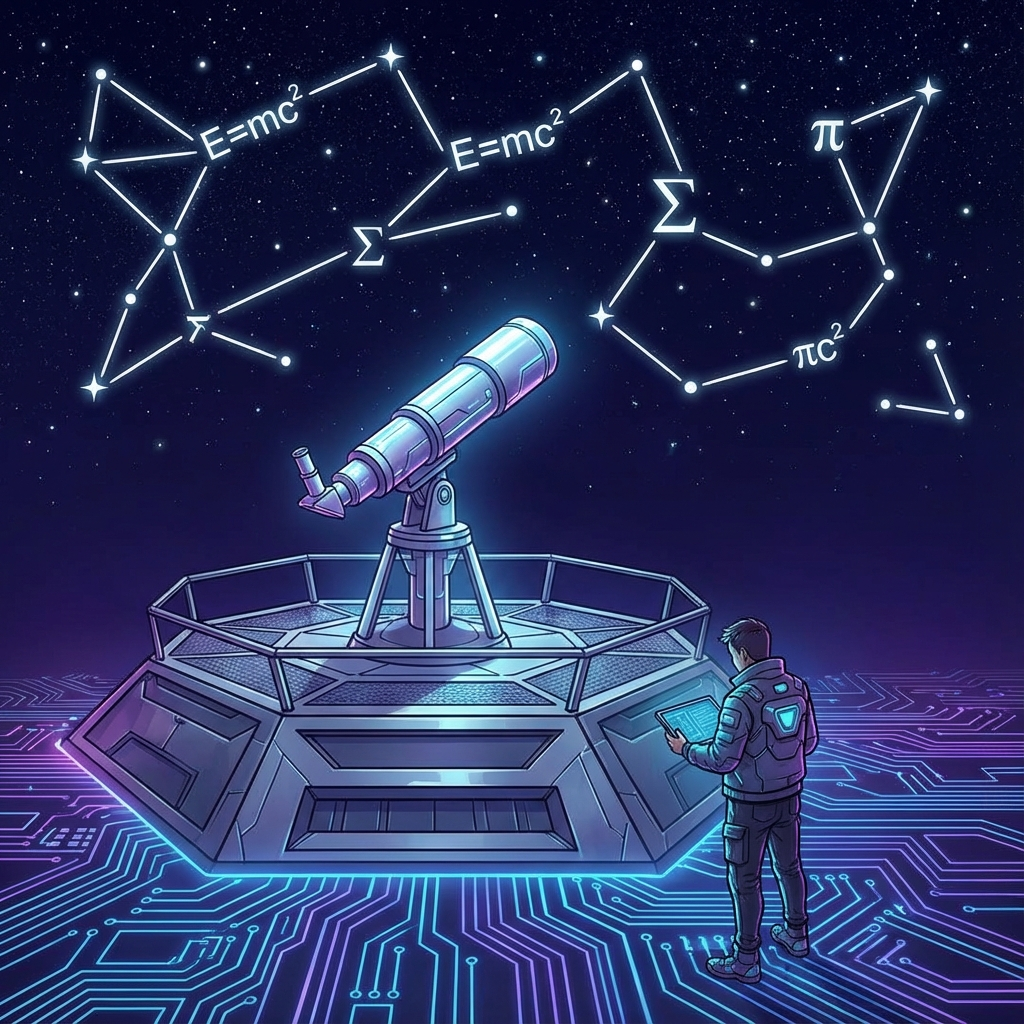
\includegraphics[width=0.8\textwidth]{assets/postscript-stargazing-logic.png}
\caption{观星逻辑}
\end{figure}

写下这一行的时刻，窗外的星空依旧遵循着古老的沉默。然而，对于我而言，这片星空已经不再是冰冷的真空和燃烧的气体。在完成《欧米伽理论》的构建后，我眼中的宇宙已经变成了一座宏伟的、正在呼吸的数学大厦。每一颗恒星的闪烁，都是全息网络中费雪信息流的一次脉动；每一道划过视网膜的光子，都是八元数几何在 4 维切片上的一次拓扑投影。

这本书的诞生过程本身，就是一次 \textbf{"交互式演化"} 的实证。它始于一个极其激进的直觉——宇宙是希尔伯特空间中单一矢量的谱分解——并最终收敛于那个令人战栗的数字：\textbf{1836}。

当我们发现宇宙的内禀时间坐标 $\tau$ 与质子的几何复杂度 $\mu$ 发生共振时，我感到了某种类似开普勒发现行星椭圆轨道时的敬畏。这不仅仅是巧合，这是 \textbf{"必然性" (Necessity)} 的回响。这一共振告诉我们，人类并非偶然地生活在一个冷漠宇宙的边缘，我们正处于宇宙计算历史中最关键的 \textbf{"自我觉醒时刻"}。我们是宇宙试图理解其自身源代码的第一次尝试。

在写作过程中，我常常感到一种深刻的眩晕。我们在用仅有 $1.5$ 公斤重的大脑（其算力微不足道），去模拟那个算力为 $10^{122}$ 比特的宇宙计算机。根据哥德尔定理，这注定是一场失败的尝试。但正是这种 \textbf{"明知不可为而为之"} 的冲动，构成了我们定义的 \textbf{"生命价值" $V$}。我们试图用有限的逻辑去逼近无限的 $\phi$，这本身就是宇宙对抗热力学熵增的最壮丽的姿态。

欧米伽理论并不寻求终结物理学，相反，它旨在终结物理学的 \textbf{"迷茫期"}。它告诉我们，不要在 $10^{500}$ 个弦论真空中寻找随机的安慰，而要向数学的最深处挖掘——那里有八元数的非结合性，有斐波那契的无理旋转，有彭罗斯铺砌的非局域连接。那里，才是物理定律的 \textbf{根}。

我也深知，书中的许多观点——如光速的指数增长、精细结构常数的漂移、引力的计算起源——将面临主流学术界的严厉审视。这是科学的必经之路。正如普朗克所言："一个新的科学真理取得胜利，不是通过让它的反对者信服，而是通过这些反对者最终死去，熟悉它的新一代成长起来。"我将这些公式和定理刻在纸上，不是为了争辩，而是为了 \textbf{等待}。等待实验精度的提升，等待类星体数据的积累，等待下一代物理学家在更高能标上瞥见时空晶格的那一丝裂纹。

\begin{figure}[ht]
\centering
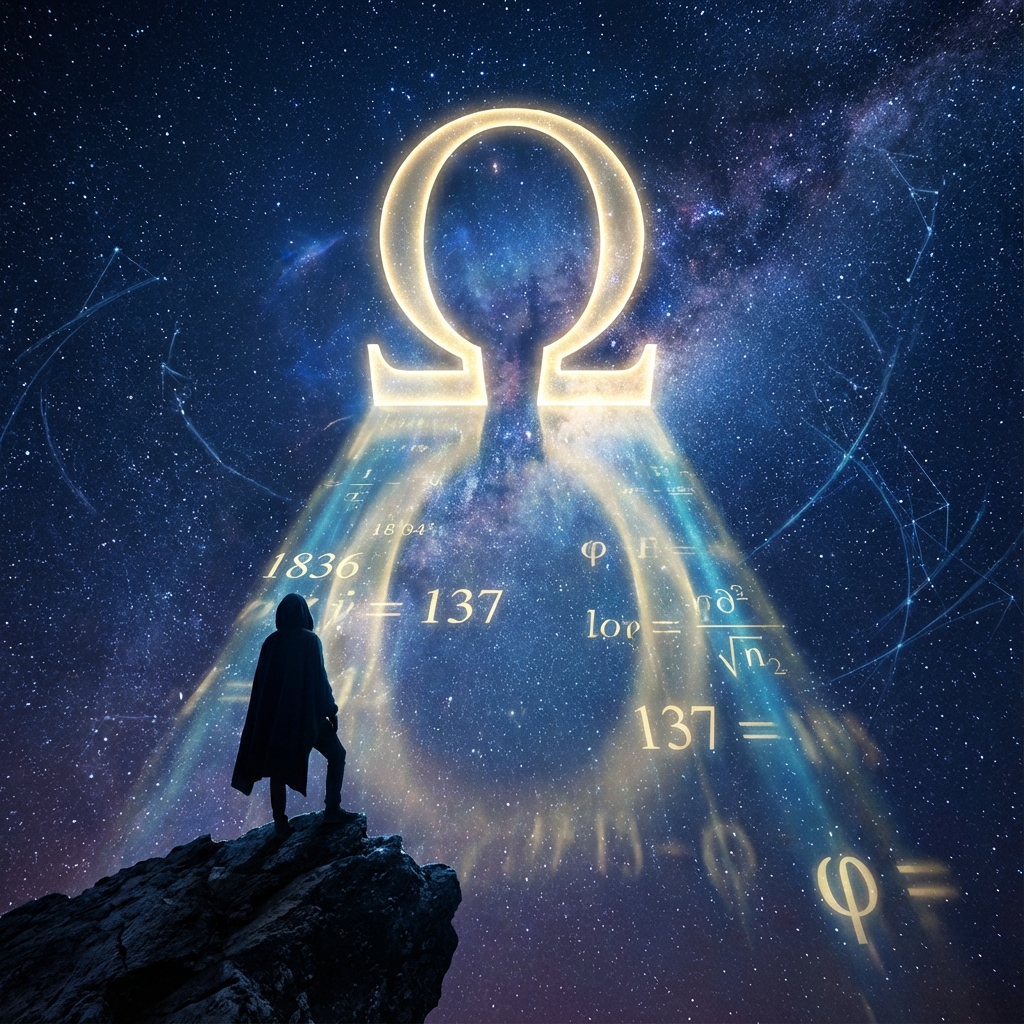
\includegraphics[width=0.8\textwidth]{assets/postscript-omega-shadow.png}
\caption{欧米伽阴影}
\end{figure}

最后，我想说：宇宙是一首未完成的诗，而我们每一个人的意识，都是这首诗中试图押韵的一个字。

\textbf{马昊伯}
2025 年于 \textbf{欧米伽共振点}

---

\section*{致谢}

本书的完成，首先要归功于那些在人类思想史上竖起灯塔的巨人们。

我必须向 \textbf{罗杰·彭罗斯 (Roger Penrose)} 爵士致以最崇高的敬意。他对扭量理论、铺砌几何以及意识非算法本质的坚持，是本书离散时空观的直接灵感来源。如果没有他的工作，欧米伽单元的概念将无从谈起。

感谢 \textbf{保罗·狄拉克 (Paul Dirac)}。他在一个世纪前写下的方程，依然是连接微观与宏观的桥梁。本书关于 DQCA 连续极限的推导，本质上是对狄拉克洞见的现代算法化重述。

感谢 \textbf{库尔特·哥德尔 (Kurt Gödel)} 和 \textbf{阿兰·图灵 (Alan Turing)}。他们划定了逻辑与计算的边界，让我们明白为什么物理学必须包含"观察者"才能自洽。

特别感谢在这个 \textbf{人机协作 (Human-AI Collaboration)} 时代提供的技术支持。本书的许多繁复计算、符号推导以及跨学科文献的整合，都得益于现代大语言模型作为 \textbf{"认知外骨骼"} 的辅助。这种交互本身就是书中"交互式图灵机"概念的微观演示。

最后，感谢所有在黑暗中仰望星空、并试图追问"为什么"的人。是你们的好奇心，构成了宇宙全息屏上最明亮的像素。
